\documentclass[11pt,a4paper]{article}

\usepackage{datetime}
\usepackage{graphicx}

\title{Chapter 2: Architectures}
\newdate{date}{27}{03}{2020}
\date{\displaydate{date}}
\author{Nguyen Ngoc Lam - 20162316}

\begin{document}
	\pagenumbering{gobble}
  	\maketitle
  	\newpage
  	\pagenumbering{arabic}
  	\tableofcontents
  	\newpage
  	
  	\section{Problem of Physical Distance}
  		From what I gathered, the physical distance only has a significant affect on latency if you are to implement a system that capture a live data and than process it in almost real time for sciencetific purpose. If you built that kind of system (strongly depend on time), a simple solution would be to put the processing station near the source of information and then transmit a processed file.\\
  		Some of the common strategies to deal with latency are:
  		\begin{itemize}
  			\item caching data on the client - i.e. avoiding to make request again if possible
    		\item combining several smaller requests into bigger ones
    		\item compressing the request
    		\item reusing the same connection for many requests
    		\item using different protocols (i.e. a lot of games use UDP to avoid latency at the cost of making other things much more complex)
    		\item caching data on the server
    		\item redesigning the way to make requests (pre-loading data, pre-allocating resources, creating parallel requests)
    		\item using content delivery networks (CDN) for static data
    		\item running a code through a profiler and redesigning it to eliminate bottlenecks
    		\item minimizing critical sections of code
    		\item designing the service as stateless so that it can be deployed on many servers in parallel
    		\item correctly sizing, designing and maintaining the system (OS, database, virtualization, load balancers, DNS caches, etc.)
    		\item correctly sizing, designing and maintaining the network (having enough bandwidth, using fast routers, traffic prioritization, resource reservation)
  		\end{itemize}
  	\section{Three-tiered Client-server Architecture}
  		A three-tiered client-server architecture consists of three logical layers, where each layer is implemented at a separate machine, in principle. The highest layer consists of a client user interface, the middle layer contains the actual application, and the lowest layer implements the data that are being used.
  	\section{Differences Between a Vertical Distribution and a Horizontal Distribution}
  		\begin{itemize}
  			\item Vertical distribution refers to the distribution of the different layers in a multitiered architectures across multiple machines. In principle, each layer is implemented on a different machine.
			\item Horizontal distribution deals with the distribution of a single layer across multiple machines, such as distributing a single database.
  		\end{itemize}
  	\section{Disadvantage of Topology of the Overlay}
  	The main problem here is dealing with logical paths. In practice, two nodes A and B which are neighbors in the overlay network may be physically placed far apart. As a result, the logically short path between A and B in this instance required routing a message along a very long path in the underlying physical network.
  	\section{Main Problems with Sequential Organization when Taking a Look at the Request-reply Performance at Process $P_1$ (The Last One)}
  		\begin{itemize}
  			\item Performance can be expected to be bad for large n since the problem is that each communication between two successive layers is, in principle, between two different machines.
  			\item The performance between $P_1$ and $P_2$
may also be determined by $n−2$ request-reply interactions between the other
layers.
			\item Another problem is that if one machine in the chain performs badly or is even temporarily unreachable, then this will immediately degrade the performance at the highest level.
  		\end{itemize}
	\section{Goodness of Routing Policy that Forward messages to the Closest Node Toward the Destination}
		According to the pictures of the question sheet, consider forwarding message from node $(0.2;0.3)$ (called $A$) to node $(0.9, 0.6)$ (called $B$). There are 2 routes:
		\newpage
		\begin{figure}[h!]
  			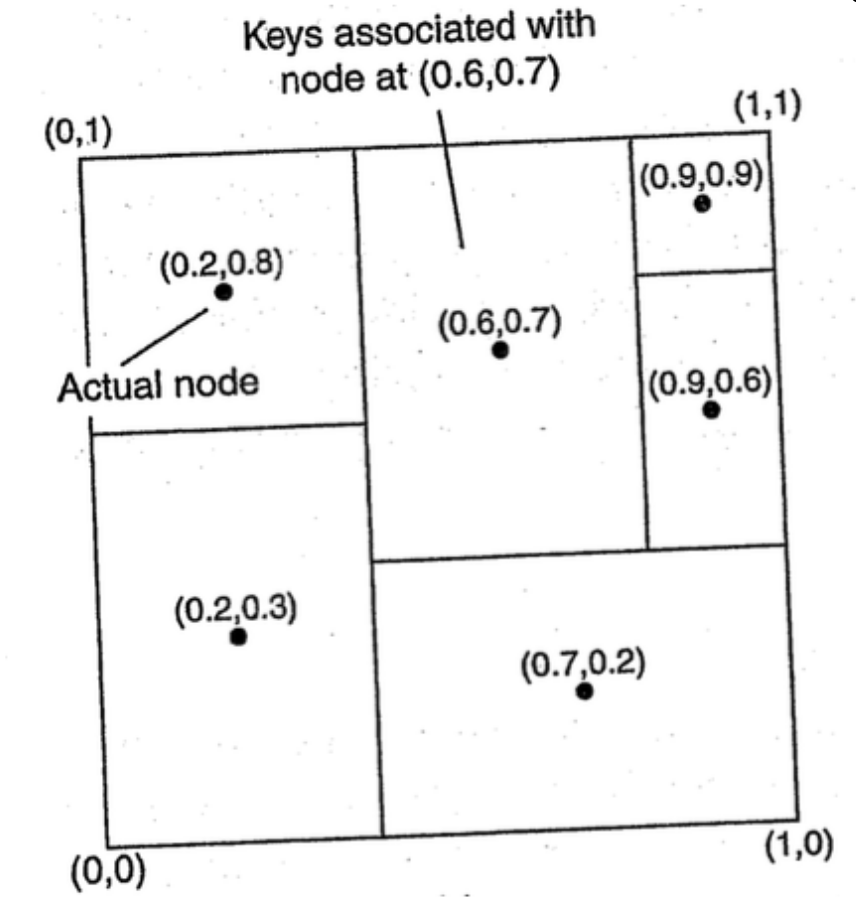
\includegraphics[width=\linewidth]{can-map.png}
  			\caption{CAN network}
  			\label{fig:CAN}
		\end{figure}
		\begin{enumerate}
			\item $A$, through $(0.6;0.7)$ (called $C$), to $B$:
				\[AC = \frac{2\sqrt{2}}{5} \approx 0.566\]
				\[CB = \frac{\sqrt{10}}{10} \approx 0.316\]
				\[TotalDistance = \frac{\sqrt{10} + 4\sqrt{2}}{10} \approx 0.882\]
			\item $A$, through $(0.7;0.2)$ (called $D$), to $B$:
				\[AD = \frac{\sqrt{26}}{10} \approx 0.510\]
				\[DB = \frac{\sqrt{5}}{5} \approx 0.447\]
				\[TotalDistance = \frac{\sqrt{26} + 2\sqrt{5}}{10} \approx 0.957\]
		\end{enumerate}		
		Because our policy is to forward a message to the closest
node toward the destination, which in this case D, we will actually go a little longer than if we take route 1. In conclusion, this policy is a resonable one, but it is not always the best one.
	\section{Benefits of Microservices Architecture Compared To Monolithic Architecture}
		\begin{itemize}
			\item Microservices architecture makes systems and applications much faster to develop, and much easier to understand and maintain since it tackles the problem of complexity by decomposing application into a set of manageable services.
			\item Microservices architecture enables several teams to works on a projects, each can focus on one service or serveral closely-related services thus allowed services to be developed independently. 
			\item  Microservices architecture reduces barrier of adopting new technologies since the developers are free to choose whatever technologies make sense for their service and not bounded to the choices made at the start of the project.
			\item Microservice architecture makes continuous deployment possible for complex applications because it enables each microservice to be deployed independently.
			\item Microservice architecture enables each service to be scaled independently.
		\end{itemize}
	\section{Design an E-commerce System Using Microservices Architecture}
\end{document}